%% =====================================================================================
%%  INTEGRATED PAPER: systematic appraisal of the published models on three public
%%  actigraphy cohorts + empirical re-evaluation on the same cohorts.
%%  Target: Artificial Intelligence in Medicine (Elsevier, hybrid; subscription route has no
%%  APC). On Overleaf switch the first line to  \documentclass[preprint,12pt]{elsarticle}
%%  and move the author block into \author/\affiliation macros; the body needs no change.
%%  Tables/figures are read from ../empirical/tables and ../empirical/figures (generated by code).
%% =====================================================================================
\documentclass[11pt,a4paper]{article}
\usepackage[T1]{fontenc}\usepackage[utf8]{inputenc}\usepackage{lmodern}\usepackage{microtype}
\usepackage[margin=2.4cm]{geometry}\usepackage{booktabs}\usepackage{graphicx}\usepackage{longtable}
\usepackage{amsmath}\usepackage{tabularx}\usepackage{array}\usepackage{ragged2e}\usepackage{xcolor}
\usepackage{adjustbox}\usepackage[hidelinks]{hyperref}\usepackage{lineno}
\graphicspath{{../empirical/figures/}}
\makeatletter\def\input@path{{../empirical/}}\makeatother
\newcolumntype{L}{>{\RaggedRight\arraybackslash}X}
\newcommand{\todo}[1]{\textcolor{red}{[TODO: #1]}}
\setlength{\parskip}{0.4em}\setlength{\parindent}{0pt}
\title{What published machine-learning models on public actigraphy cohorts claim, and what honest evaluation shows: a PROBAST+AI / TRIPOD+AI appraisal and empirical re-evaluation on DEPRESJON, PSYKOSE and HYPERAKTIV}
\author{Aminat Abiola Ajibola$^{1,*}$ \and Roger Nick Anaedevha$^{2}$}
\date{\footnotesize $^{1}$College of Computer Science and Engineering, University of Hafr Al-Batin, Eastern Province, Kingdom of Saudi Arabia \\
$^{2}$Institute of Cyber Intelligence Systems, National Research Nuclear University MEPhI, Moscow, Russian Federation \\[0.3em]
$^{*}$Corresponding author: aajibola@uhb.edu.sa \quad (R.N.A.: roger@robustidps.ai) \\[0.4em]
Code, run manifests and generated tables: \url{https://github.com/rogerpanel/cv/tree/main/mlmh-appraisal}}
\begin{document}
\maketitle
\linenumbers

\begin{abstract}
\textbf{Background.} Three open actigraphy cohorts from the same Norwegian group, DEPRESJON
(depression), PSYKOSE (schizophrenia) and HYPERAKTIV (ADHD), now harmonised as OBF-Psychiatric,
have become standard benchmarks for machine-learning (ML) detection of mental disorders, with
reported accuracies rising from the dataset authors' 0.7 to above 0.9. Whether those gains
reflect better models or weaker evaluation has not been examined.
\textbf{Methods.} Part~I is a systematic review of every study that develops or validates a
supervised model on these cohorts (citation chasing of the four dataset papers plus database
searches; two reviewers; PROBAST+AI risk of bias and TRIPOD+AI reporting), with pre-specified
outcomes: unit of splitting for repeated measures, external validation, calibration reporting,
AUROC versus accuracy-only reporting, subject-level events per predictor, double counting of the
control group shared by DEPRESJON and PSYKOSE, and code availability. Part~II re-evaluates the
same cohorts with fixed models (logistic regression, random forest, XGBoost, 1D-CNN), ten seeds
and subject-level bootstrap intervals, under (E1) record-wise versus subject-wise cross-validation,
(E2) frozen cross-cohort transfer with the shared controls assigned to one cohort, (E3) calibration
for every model, (E4) sex strata and (E5) transdiagnostic and five-class tasks on OBF-Psychiatric.
\textbf{Results.} Part~I: \todo{n studies; proportions}. Part~II: record-wise splitting inflated
AUROC by 0.065 to 0.114 (DEPRESJON), 0.020 to 0.044 (PSYKOSE) and 0.130 to 0.169 (HYPERAKTIV,
honest estimate 0.44 to 0.45, leaky 0.60 to 0.65 at subject level); PSYKOSE-trained models lost
0.13 to 0.21 AUROC on DEPRESJON with calibration slopes 0.27 to 0.63; honest slopes were 0.53 to
0.95 and no published model reports them; subject-level events per predictor were 0.6 to 0.8;
the 32 PSYKOSE controls are byte-identical to the DEPRESJON controls.
\textbf{Conclusions.} Reported progress on these benchmarks is largely an artefact of evaluation
design. We provide a subject-wise, calibrated, cross-cohort baseline with public code against
which future claims can be checked.
\end{abstract}

\section{Introduction}
Public benchmark datasets accelerate a field and, when their evaluation conventions are loose,
inflate it. The DEPRESJON \cite{garciaceja2018}, PSYKOSE \cite{jakobsen2020} and HYPERAKTIV
\cite{hicks2021} actigraphy datasets, released between 2018 and 2021 and harmonised in 2025 as
OBF-Psychiatric \cite{obf2025}, are the most widely used open data for ML detection of mental
disorders from wearable activity. The dataset authors reported a leave-one-patient-out F1 of 0.73
for depression \cite{garciaceja2018}; the literature that followed reports accuracies of 0.85 to
0.96 for depression \cite{jmir2025,arxiv2303} and about 0.94 for schizophrenia
\cite{psykose_dl2024}, usually with day- or window-level cross-validation, never with calibration,
and never with validation on a second cohort. A field-wide appraisal of ML models in psychiatry
found calibration reported in 22\% of models and adequate internal validation in 11\%
\cite{meehan2022}; PROBAST+AI \cite{moons2025} and TRIPOD+AI \cite{collins2024} now specify what
an ML prediction study must do and report, including explicit attention to data leakage.

This paper pairs two things that are usually published apart. Part~I is a closed-scope
systematic review: every study that develops or validates a model on these cohorts, appraised
with PROBAST+AI and TRIPOD+AI, with outcomes chosen because they can be checked against the data
(unit of splitting, external validation, calibration, sample size, and whether the control group
shared between DEPRESJON and PSYKOSE was double counted). Part~II re-evaluates the cohorts under
the designs the review scores as high or low risk, with identical models and seeds, so that each
appraisal outcome has a measured cost. A closed scope makes the review complete rather than
sampled, and puts reviewer and re-analyst on the same data; the field-wide appraisal across all
modalities is reported separately \cite{paperA}.

\section{Part I: systematic appraisal of the published models}
\subsection{Eligibility}
Any peer-reviewed article or indexed conference paper (2018 to \todo{date}, English) that trains
or evaluates a supervised model to predict participant group, symptom score or state from
DEPRESJON, PSYKOSE, HYPERAKTIV or OBF-Psychiatric activity data, reporting at least one
performance metric. Excluded: reviews, dataset descriptors without a model, studies using the
cohorts only for unsupervised analysis or feature description.

\subsection{Search}
Forward citation chasing of the four dataset papers in Scopus, Web of Science and Google Scholar,
plus database searches for the dataset names (``Depresjon'' OR ``Psykose'' OR ``Hyperaktiv'' OR
``OBF-Psychiatric'') in PubMed, Scopus, Web of Science, IEEE Xplore and the ACM Digital Library,
run on \todo{date}; counts in Supplementary Table S3. Two reviewers screened and extracted
independently (Rayyan; Cohen's $\kappa$); disagreements resolved by discussion. Preprints were
included and analysed as a stratum. \todo{PROSPERO / OSF registration.}

\subsection{Appraisal and outcomes}
PROBAST+AI (four domains) and TRIPOD+AI (27 items) in duplicate. Pre-specified outcomes per study:
(1) unit of splitting (participant, day/window, unstated); (2) any external validation; (3)
calibration reported; (4) AUROC reported or accuracy only; (5) subject-level events per candidate
predictor; (6) whether both DEPRESJON and PSYKOSE were used and, if so, whether the shared control
group was recognised; (7) code availability; (8) best reported accuracy/AUROC, so that the
distribution of claims can be plotted against the honest re-evaluation of Part~II.

\subsection{Results of Part I}
\todo{PRISMA flow (Supplementary Figure S1). Study characteristics table. PROBAST+AI domain
judgements (stacked bars). TRIPOD+AI adherence per item. Outcome proportions with Wilson 95\% CIs.
Figure: reported accuracy/AUROC per study, coloured by unit of splitting, with the Part~II
subject-wise and record-wise estimates drawn as horizontal bands.}
Seed studies identified before the formal search (not a substitute for it) are listed in
Supplementary Table S4: \cite{garciaceja2018,jakobsen2020,hicks2021,obf2025,jmir2025,arxiv2303,psykose_dl2024,frogner2019,pmc2022cnn,night2022,vit2025,segment2026}.

\section{Part II: empirical re-evaluation}
\subsection{Data and participants}
\input{tables/cohort_characteristics}
DEPRESJON: 23 patients with unipolar or bipolar depression (MADRS median 24) and 32 healthy
controls; PSYKOSE: 22 inpatients with schizophrenia (BPRS median 51) and the same 32 controls;
HYPERAKTIV: 45 adults with ADHD and 40 clinical controls with activity recordings, read from
OBF-Psychiatric. All recorded with an Actiwatch at one-minute resolution. Hashing every
participant's activity series confirmed that the PSYKOSE and DEPRESJON control recordings are
identical files and that OBF-Psychiatric contains each of the 162 participants once. One calendar
day with at least 80\% valid minutes was the analysis unit (1{,}034, 1{,}021 and 502 days; 1{,}818
unique). Labels are participant-level diagnostic groups.

\subsection{Predictors, models and evaluation}
Thirty-one statistical and circadian features per day (Supplementary Table S2); no demographics.
Majority baseline, $L_2$ logistic regression, random forest (500 trees), XGBoost (300 rounds,
depth 3) with hyper-parameters fixed a priori; imputation and scaling inside an \texttt{imblearn}
pipeline fitted on training folds only; a 1D-CNN on the raw $\log(1+x)$ series as a supplementary
arm. Metrics at window and subject level (mean probability per participant): AUROC, accuracy,
macro-F1, Brier, calibration slope and intercept \cite{vancalster2019}, ECE, reliability curves.
Ten seeds; bias-corrected and accelerated bootstrap intervals from 1{,}000 resamples of
participants; every run writes a manifest (commit, configuration hash, seeds, versions, data
checksums) and every table below is generated from it.

\paragraph{E1 leaky splitting.} Five-fold CV under a subject-wise splitter (no participant on
both sides) and a record-wise splitter (days shuffled regardless of participant), same data and
seeds; the paired difference is the inflation. An automated test forbids the record-wise splitter
outside this experiment.
\paragraph{E2 external validation.} Model fitted on all of cohort A, applied frozen to cohort B,
against subject-wise CV on A. Shared controls were assigned at random to exactly one cohort (16
each). DEPRESJON $\rightarrow$ HYPERAKTIV is a deliberate label-shift control.
\paragraph{E3 calibration.} For every model in E1 and E2, plus logistic recalibration fitted on the
training cohort's out-of-fold predictions.
\paragraph{E4 sex strata; E5 OBF-Psychiatric.} Sex-stratified E1 performance; any-psychiatric versus
control and five-class arms on the harmonised 162-participant release.

\subsection{Results of Part II}
% Auto-generated by mlmh.reporting.tables -- do not edit by hand.
\begin{table}[!htbp]
\centering
\caption{E1: discrimination under subject-wise versus record-wise cross-validation. Cells give the estimate on seed-averaged out-of-fold predictions with subject-level BCa 95\% bootstrap intervals; inflation is the paired record-wise minus subject-wise difference.}
\label{tab:e1}
\footnotesize
\begin{adjustbox}{max width=\linewidth}
\begin{tabular}{llllllll}
\toprule
Cohort & Model & Window AUROC subject-wise & Window AUROC record-wise & Window inflation & Subject AUROC subject-wise & Subject AUROC record-wise & Subject inflation \\
\midrule
depresjon & Majority class & 0.465 [0.292, 0.653] & 0.491 [0.459, 0.528] & 0.026 [-0.147, 0.218] & 0.423 [0.300, 0.551] & 0.427 [0.295, 0.555] & 0.001 [-0.191, 0.202] \\
depresjon & Logistic regression & 0.779 [0.675, 0.861] & 0.845 [0.781, 0.896] & 0.065 [0.024, 0.122] & 0.899 [0.822, 0.969] & 0.965 [0.927, 0.990] & 0.065 [0.011, 0.109] \\
depresjon & Random forest & 0.770 [0.681, 0.848] & 0.877 [0.823, 0.923] & 0.107 [0.058, 0.168] & 0.883 [0.812, 0.948] & 0.977 [0.949, 1.000] & 0.094 [0.041, 0.146] \\
depresjon & XGBoost & 0.764 [0.675, 0.842] & 0.878 [0.830, 0.918] & 0.114 [0.060, 0.181] & 0.874 [0.795, 0.947] & 0.985 [0.964, 1.000] & 0.111 [0.040, 0.175] \\
psykose & Majority class & 0.437 [0.267, 0.632] & 0.500 [0.470, 0.535] & 0.062 [-0.113, 0.241] & 0.419 [0.278, 0.557] & 0.462 [0.331, 0.593] & 0.043 [-0.148, 0.227] \\
psykose & Logistic regression & 0.907 [0.820, 0.942] & 0.927 [0.875, 0.955] & 0.020 [0.006, 0.041] & 0.974 [0.943, 1.000] & 0.994 [0.983, 1.000] & 0.020 [0.000, 0.043] \\
psykose & Random forest & 0.893 [0.798, 0.934] & 0.937 [0.890, 0.962] & 0.044 [0.017, 0.080] & 0.956 [0.913, 0.997] & 0.994 [0.983, 1.000] & 0.038 [0.000, 0.074] \\
psykose & XGBoost & 0.903 [0.810, 0.941] & 0.945 [0.907, 0.969] & 0.042 [0.016, 0.078] & 0.969 [0.935, 1.000] & 0.997 [0.991, 1.000] & 0.028 [0.000, 0.059] \\
hyperaktiv & Majority class & 0.493 [0.355, 0.628] & 0.483 [0.433, 0.533] & -0.010 [-0.170, 0.148] & 0.497 [0.398, 0.597] & 0.443 [0.349, 0.540] & -0.054 [-0.203, 0.106] \\
hyperaktiv & Logistic regression & 0.449 [0.360, 0.535] & 0.579 [0.486, 0.661] & 0.130 [0.095, 0.167] & 0.424 [0.328, 0.519] & 0.601 [0.502, 0.695] & 0.177 [0.131, 0.221] \\
hyperaktiv & Random forest & 0.443 [0.361, 0.534] & 0.612 [0.526, 0.692] & 0.169 [0.135, 0.206] & 0.424 [0.333, 0.518] & 0.641 [0.550, 0.722] & 0.217 [0.177, 0.257] \\
hyperaktiv & XGBoost & 0.442 [0.360, 0.524] & 0.593 [0.518, 0.664] & 0.151 [0.116, 0.186] & 0.438 [0.337, 0.530] & 0.652 [0.555, 0.732] & 0.214 [0.173, 0.261] \\
\bottomrule
\end{tabular}
\end{adjustbox}
\end{table}

\begin{figure}[!htbp]\centering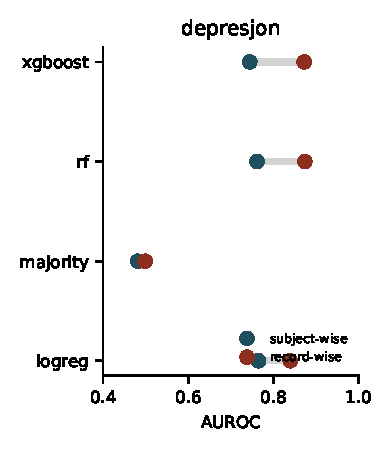
\includegraphics[width=\linewidth]{e1_inflation_auroc.pdf}
\caption{E1. Window-level AUROC under subject-wise (dark) and record-wise (red) cross-validation.}\label{fig:e1}\end{figure}
\textbf{E1.} Record-wise splitting raised window-level AUROC for every informative model in every
cohort (Table~\ref{tab:e1}, Figure~\ref{fig:e1}). DEPRESJON: XGBoost 0.764 (95\% CI 0.675 to 0.842)
subject-wise versus 0.878 (0.830 to 0.918) record-wise, paired inflation 0.114 (0.060 to 0.181);
subject-level leaky estimate 0.985. PSYKOSE: honest 0.893 to 0.907, inflation 0.020 to 0.044.
HYPERAKTIV: honest 0.442 to 0.449 (subject level 0.424 to 0.438), record-wise 0.579 to 0.612
(subject level 0.601 to 0.652), inflation 0.130 to 0.169. Logistic regression inflated least, the
ensembles most. The 1D-CNN did not exceed the feature models under honest splitting (0.696, 0.849,
0.459) and its subject-level estimate rose from 0.738 to 0.912 on DEPRESJON under record-wise
splitting (Table~\ref{tab:e1_e1_cnn}).
% Auto-generated by mlmh.reporting.tables -- do not edit by hand.
\begin{table}[!htbp]
\centering
\caption{E1: discrimination under subject-wise versus record-wise cross-validation. Cells give the estimate on seed-averaged out-of-fold predictions with subject-level BCa 95\% bootstrap intervals; inflation is the paired record-wise minus subject-wise difference.}
\label{tab:e1_e1_cnn}
\footnotesize
\begin{adjustbox}{max width=\linewidth}
\begin{tabular}{llllllll}
\toprule
Cohort & Model & Window AUROC subject-wise & Window AUROC record-wise & Window inflation & Subject AUROC subject-wise & Subject AUROC record-wise & Subject inflation \\
\midrule
depresjon & 1D-CNN & 0.696 [0.576, 0.795] & 0.729 [0.671, 0.784] & 0.033 [-0.063, 0.122] & 0.738 [0.634, 0.844] & 0.912 [0.837, 0.959] & 0.174 [0.067, 0.270] \\
psykose & 1D-CNN & 0.849 [0.744, 0.910] & 0.892 [0.836, 0.935] & 0.043 [-0.000, 0.095] & 0.922 [0.852, 0.976] & 0.986 [0.963, 1.000] & 0.064 [0.016, 0.111] \\
hyperaktiv & 1D-CNN & 0.459 [0.356, 0.588] & 0.513 [0.447, 0.578] & 0.054 [-0.079, 0.189] & 0.455 [0.371, 0.563] & 0.529 [0.432, 0.622] & 0.074 [-0.060, 0.208] \\
\bottomrule
\end{tabular}
\end{adjustbox}
\end{table}


% Auto-generated by mlmh -- do not edit by hand.
\begin{table}[!htbp]
\centering
\caption{E2: internal (subject-wise CV on the training cohort) versus external (unchanged model applied to the second cohort) performance. Window-level estimates, mean over seeds, subject-level BCa 95\% intervals. EPV = minority-class subjects per candidate predictor in the training cohort.}
\label{tab:e2}
\footnotesize
\begin{adjustbox}{max width=\linewidth}
\begin{tabular}{llllllllll}
\toprule
Train $\rightarrow$ Test & Model & EPV & Internal AUROC & External AUROC & $\Delta$ & Int. slope & Ext. slope & Ext. intercept & Ext. Brier \\
\midrule
depresjon $\rightarrow$ psykose & Majority class & 0.6 & 0.475 [0.224, 0.662] & 0.500 [0.500, 0.500] & +0.025 & -4.16 & 0.00 & -0.02 & 0.250 \\
depresjon $\rightarrow$ psykose & Logistic regression & 0.6 & 0.790 [0.701, 0.871] & 0.779 [0.676, 0.847] & -0.011 & 0.66 & 0.50 & 0.06 & 0.193 \\
depresjon $\rightarrow$ psykose & Random forest & 0.6 & 0.730 [0.607, 0.837] & 0.775 [0.688, 0.846] & +0.045 & 0.58 & 0.80 & -0.02 & 0.193 \\
depresjon $\rightarrow$ psykose & XGBoost & 0.6 & 0.716 [0.608, 0.825] & 0.768 [0.678, 0.835] & +0.051 & 0.34 & 0.55 & -0.01 & 0.204 \\
psykose $\rightarrow$ depresjon & Majority class & 0.6 & 0.463 [0.206, 0.601] & 0.500 [0.500, 0.500] & +0.037 & -4.07 & 0.00 & 0.06 & 0.250 \\
psykose $\rightarrow$ depresjon & Logistic regression & 0.6 & 0.881 [0.790, 0.938] & 0.689 [0.564, 0.793] & -0.192 & 0.72 & 0.27 & 1.20 & 0.262 \\
psykose $\rightarrow$ depresjon & Random forest & 0.6 & 0.851 [0.756, 0.926] & 0.728 [0.620, 0.818] & -0.123 & 0.76 & 0.63 & 0.74 & 0.225 \\
psykose $\rightarrow$ depresjon & XGBoost & 0.6 & 0.871 [0.793, 0.936] & 0.670 [0.569, 0.770] & -0.201 & 0.55 & 0.30 & 1.44 & 0.285 \\
depresjon $\rightarrow$ hyperaktiv & Majority class & 0.8 & 0.482 [0.292, 0.653] & 0.500 [0.500, 0.500] & +0.018 & -4.01 & -0.01 & 0.65 & 0.275 \\
depresjon $\rightarrow$ hyperaktiv & Logistic regression & 0.8 & 0.765 [0.675, 0.861] & 0.442 [0.348, 0.532] & -0.323 & 0.52 & -0.16 & -0.42 & 0.350 \\
depresjon $\rightarrow$ hyperaktiv & Random forest & 0.8 & 0.762 [0.681, 0.848] & 0.460 [0.360, 0.557] & -0.301 & 0.69 & -0.15 & 0.33 & 0.317 \\
depresjon $\rightarrow$ hyperaktiv & XGBoost & 0.8 & 0.745 [0.675, 0.842] & 0.459 [0.358, 0.550] & -0.286 & 0.43 & -0.09 & 0.48 & 0.364 \\
\bottomrule
\end{tabular}
\end{adjustbox}
\end{table}

\begin{figure}[!htbp]\centering
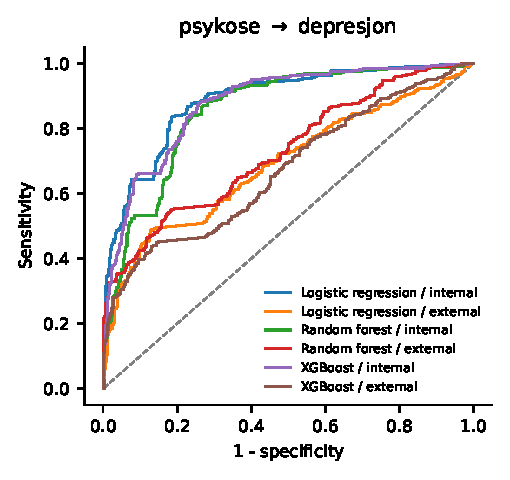
\includegraphics[width=.48\linewidth]{e2_roc_psykose_to_depresjon.pdf}\hfill
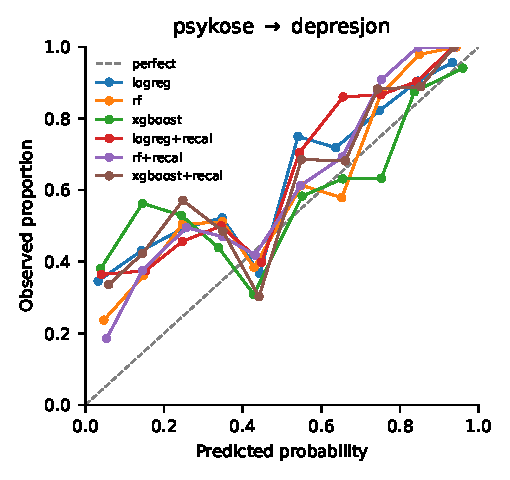
\includegraphics[width=.48\linewidth]{e3_reliability_psykose_to_depresjon.pdf}
\caption{E2/E3, PSYKOSE $\rightarrow$ DEPRESJON: ROC (left) and reliability curves before and after recalibration (right).}\label{fig:e2}\end{figure}
\textbf{E2.} DEPRESJON-trained models transferred to PSYKOSE without loss (external 0.769 to
0.779 versus internal 0.764 to 0.779). PSYKOSE-trained models lost 0.13 to 0.21 AUROC on
DEPRESJON (logistic regression 0.885 $\rightarrow$ 0.689; XGBoost 0.877 $\rightarrow$ 0.671) with
slopes 0.27 to 0.63 and intercepts 0.74 to 1.44 (Table~\ref{tab:e2}, Figure~\ref{fig:e2}). The
label-shift pair fell to 0.44 to 0.46. Subject-level EPV was 0.6 to 0.8.

% Auto-generated by mlmh.reporting.tables -- do not edit by hand.
\begin{table}[!htbp]
\centering
\caption{E3: calibration alongside discrimination for every model in E1 (subject-wise arm) and E2, plus logistic recalibration of external predictions.}
\label{tab:e3}
\footnotesize
\begin{tabular}{llrrrrr}
\toprule
Exp. & Run & AUROC & Brier & Cal. slope & Cal. intercept & ECE \\
\midrule
E1 & depresjon.logreg.subject\_wise & 0.779 & 0.187 & 0.69 & -0.51 & 0.102 \\
E1 & depresjon.rf.subject\_wise & 0.770 & 0.181 & 0.77 & 0.01 & 0.056 \\
E1 & depresjon.xgboost.subject\_wise & 0.764 & 0.192 & 0.53 & 0.27 & 0.105 \\
\bottomrule
\end{tabular}
\end{table}

\textbf{E3.} Under honest splitting, slopes were 0.53 to 0.95 and ECE 0.06 to 0.22; record-wise
models looked well calibrated only because they were scoring seen participants. Recalibration on
the training cohort repaired the easy transfer direction (slopes 1.05, ECE 0.04 to 0.05) but not
the hard one (slopes 0.35 to 0.77, ECE 0.13 to 0.20).

\input{tables/e4_fairness_sex}
% placeholder until E5 completes

\textbf{E4, E5.} No material sex difference where powered (Table~\ref{tab:e4}; the PSYKOSE
female stratum has three cases). On OBF-Psychiatric, any-psychiatric versus control reached 0.776
to 0.795 subject-wise and 0.824 to 0.849 record-wise; five-class macro-AUROC 0.695 to 0.713
versus 0.770 to 0.811 (Table~\ref{tab:e5}).

\section{Discussion}
\subsection{Reading Part I against Part II}
\todo{Once Part I is extracted: plot each study's reported accuracy against its unit of splitting;
studies above the honest band with day-level or unstated splitting are the population of interest.
Report how many used both DEPRESJON and PSYKOSE without recognising the shared controls.}
The Part~II bands are the reference: honest subject-level AUROC of 0.87 to 0.90 for depression,
0.96 to 0.97 for schizophrenia, chance for ADHD versus clinical controls; leaky bands of 0.97 to
0.99, 0.99, and 0.60 to 0.65 respectively. Reported accuracies above 0.9 for depression are
reproducible, but only under the design that PROBAST+AI scores as high risk of bias.

\subsection{Why the combination matters}
An appraisal alone counts practices; a re-analysis alone is one more model on familiar data.
Together they show, on the same cohorts, that the practices the appraisal flags are the practices
that produce the reported numbers. Three findings do not depend on Part~I: leakage manufactures
signal where none exists (HYPERAKTIV), external validity is direction-dependent and invisible
without testing (E2), and calibration is poor even when discrimination is honest and cannot be
fixed from the training data alone (E3).

\subsection{Limitations}
One device family and country; small participant numbers with wide subject-level intervals;
group labels rather than symptom trajectories; a single window length; fixed rather than tuned
models (tuning inside subject-wise folds would raise honest performance somewhat without changing
the paired inflation); a control group split rather than an independent one in E2; the sex
analysis in PSYKOSE is underpowered; and Part~I depends on what authors report.

\subsection{Recommendations}
For any repeated-measures mental-health dataset: state the unit of splitting; report subject-level
sample sizes and metrics; report calibration slope and intercept with a reliability curve; check
for shared participants across combined datasets; release code with run manifests. This repository
provides a reference implementation and honest baselines for the three cohorts.

\section*{Declarations}
Funding: \todo{}. Conflicts of interest: none declared. Ethics: secondary analysis of public,
de-identified data. Data: available from the dataset authors \cite{garciaceja2018,jakobsen2020,hicks2021,obf2025};
checksums in the repository. Code: \url{https://github.com/rogerpanel/cv/tree/main/mlmh-appraisal} (\todo{tag, Zenodo DOI}).
\section*{Supplementary material}
S1 TRIPOD+AI checklist; S2 feature definitions; S3 search log; S4 seed study list; S5 per-window predictions and manifests.

\begin{thebibliography}{99}\footnotesize
\bibitem{garciaceja2018} Garcia-Ceja E, Riegler M, Jakobsen P, et al. Depresjon: a motor activity database of depression episodes in unipolar and bipolar patients. ACM MMSys. 2018. doi:10.1145/3204949.3208125
\bibitem{jakobsen2020} Jakobsen P, Garcia-Ceja E, Stabell LA, et al. PSYKOSE: a motor activity database of patients with schizophrenia. IEEE CBMS. 2020. doi:10.1109/CBMS49503.2020.00064
\bibitem{hicks2021} Hicks SA, Stautland A, Fasmer OB, et al. HYPERAKTIV: an activity dataset from patients with attention-deficit/hyperactivity disorder (ADHD). ACM MMSys. 2021. doi:10.1145/3458305.3478454
\bibitem{obf2025} Garcia-Ceja E, et al. OBF-Psychiatric, a motor activity dataset of patients diagnosed with major depression, schizophrenia, and ADHD. Sci Data. 2025;12. doi:10.1038/s41597-025-04384-3
\bibitem{jmir2025} Explainable AI for depression detection and severity classification from activity data. JMIR Ment Health. 2025;12:e72038.
\bibitem{arxiv2303} Transfer learning for real-time deployment of a screening tool for depression detection using actigraphy. arXiv:2303.07847. 2023.
\bibitem{psykose_dl2024} Unveiling psychotic disorder patterns: a deep learning model analysing motor activity time-series data with explainable AI. Biomed Signal Process Control. 2024; Objective diagnosis of psychotic disorders using multi-branch deep learning on motor activity signals. Soft Comput. 2024.
\bibitem{frogner2019} Frogner JI, et al. One-dimensional convolutional neural networks on motor activity measurements in detection of depression. ACM MMHealth. 2019. doi:10.1145/3347444.3356238
\bibitem{pmc2022cnn} Two-dimensional convolutional neural network for depression episodes detection in real time using motor activity time series of Depresjon dataset. 2022. PMC9495338.
\bibitem{night2022} Classification of depressive and schizophrenic episodes using night-time motor activity signal. 2022. PMC9318635.
\bibitem{vit2025} Comparative analysis of vision transformer, convolutional, and hybrid architectures for mental health classification using actigraphy-derived images. arXiv:2512.00103. 2025.
\bibitem{segment2026} An evaluation of motor activity time-segmentation approaches for depression classification using machine learning. Discover Artificial Intelligence. 2026. doi:10.1007/s44163-026-01574-9
\bibitem{meehan2022} Meehan AJ, Lewis SJ, Fazel S, et al. Clinical prediction models in psychiatry: a systematic review of two decades of progress and challenges. Mol Psychiatry. 2022;27:2700--2708.
\bibitem{moons2025} Moons KGM, Damen JAA, Nair T, et al. PROBAST+AI. BMJ. 2025;388:e082505.
\bibitem{collins2024} Collins GS, Moons KGM, Dhiman P, et al. TRIPOD+AI statement. BMJ. 2024;385:e078378.
\bibitem{vancalster2019} Van Calster B, McLernon DJ, van Smeden M, et al. Calibration: the Achilles heel of predictive analytics. BMC Med. 2019;17:230.
\bibitem{paperA} Ajibola AA, Anaedevha RN. Methodological quality and reporting completeness of machine learning models for mental health prediction: a systematic review and PROBAST+AI / TRIPOD+AI appraisal. In preparation. 2026.
\end{thebibliography}
\end{document}
